\section{Contributions and Thesis Outline}
\label{sec:contributions_outline}

In the following, we briefly introduce the main contributions of this thesis addressing the clinical translation challenges of continuous neurocognitive assessments in pediatric \gls{ADHD}. They are summarized in Figure \ref{fig:contributions}.

\begin{figure}[htpb]
    \centering
    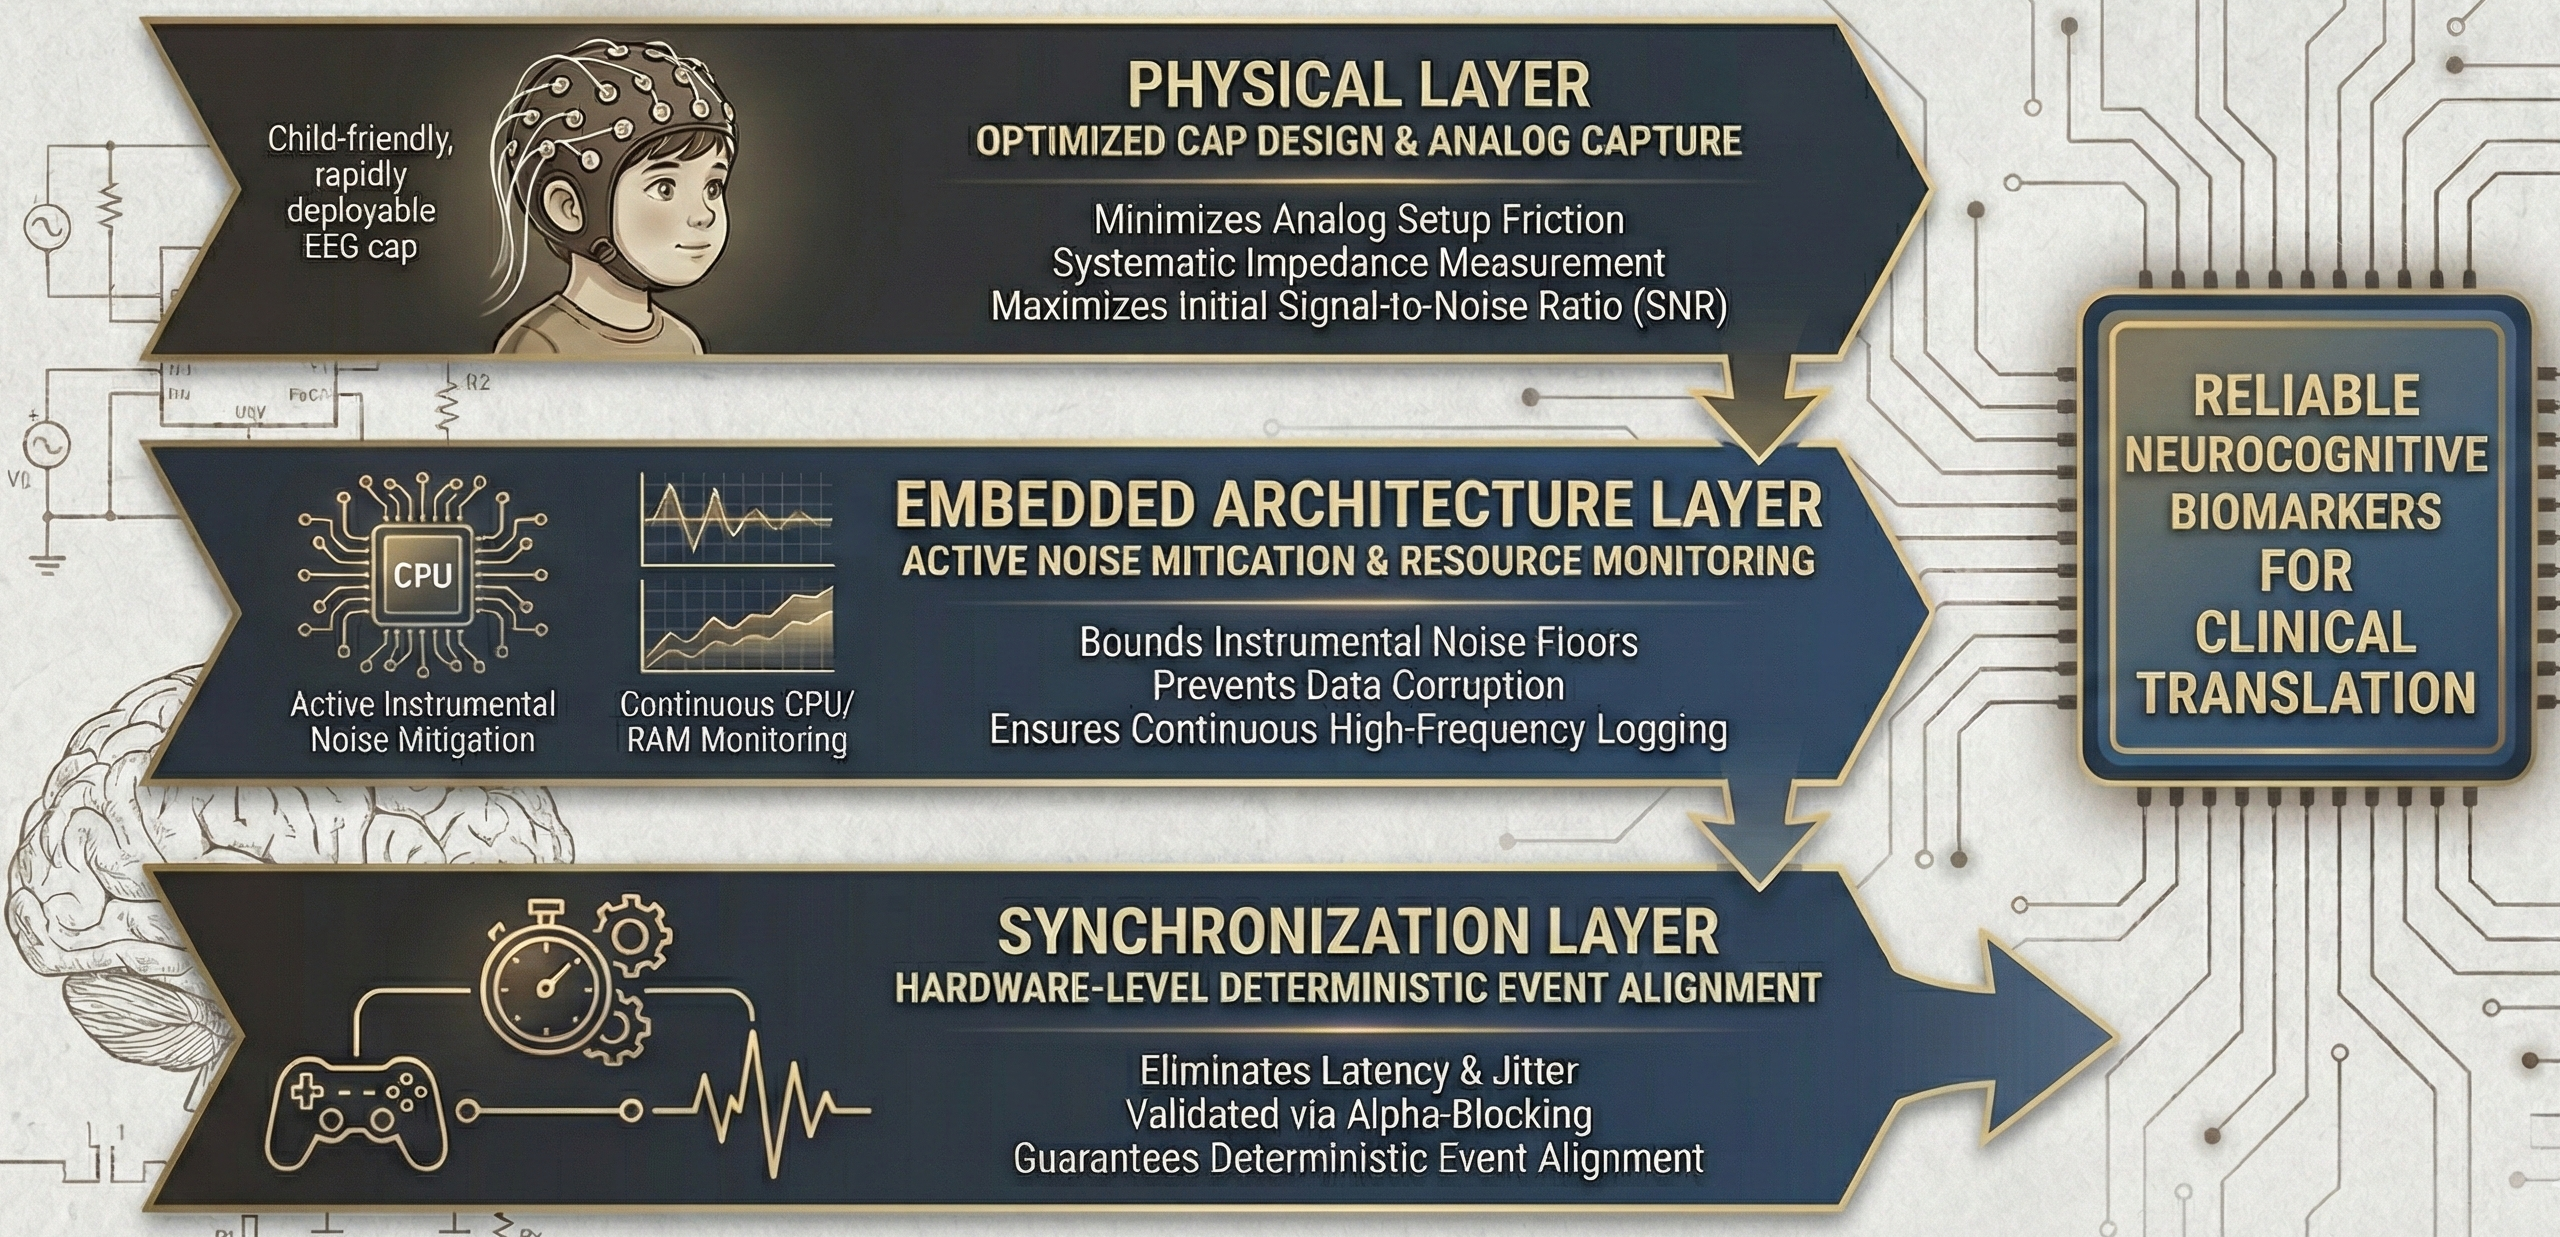
\includegraphics[width=0.8\textwidth]{Cap_1/Figures/contributions.png}
    \caption{These three core contributions form a sequential, interdependent architecture designed to secure neurocognitive data validity. The architecture begins at the \textit{Physical Layer} to secure a pristine baseline signal, passes to the \textit{Embedded Architecture Layer} for noise mitigation and resource management, and concludes in the \textit{Synchronization Layer} to guarantee deterministic event alignment.}
    \label{fig:contributions}
\end{figure}

These core contributions form a sequential, interdependent architecture designed to secure neurocognitive data validity. As illustrated in Figure \ref{fig:contributions}, only when all three sequential layers operate without failure can clinically valid Event-Related Potentials (\glspl{ERP}) be extracted for accurate \gls{ADHD} assessment.

\subsection{Optimized Physical Interface and Analog Capture}

A qualified tool for clinical neurocognitive assessments must overcome physical deployment barriers, especially when dealing with pediatric patients. The architecture begins at the physical layer, where minimizing analog setup friction is required to secure a pristine baseline signal.

Bearing this in mind, we propose a novel, rapidly deployable \gls{EEG} cap design and a systematic electrode-skin impedance measurement protocol. This development overcomes physical barriers and maximizes the initial signal-to-noise ratio (\gls{SNR}), ensuring high-fidelity analog input for the subsequent acquisition stages.

\subsection{Robust Embedded Acquisition Architecture}

The continuous, high-frequency logging of neurophysiological data is highly susceptible to instrumental noise and computational bottlenecks, which can lead to data loss or corruption during continuous assessments.

To mitigate these issues, this work presents the design and implementation of a robust \gls{EEG} acquisition system. This embedded architecture features active instrumental noise mitigation to bound noise floors, alongside continuous system-level resource monitoring (CPU and RAM) to prevent data loss. This layer ensures that the high-fidelity analog input is properly digitized and managed without corruption.

\subsection{Hardware-Level Temporal Synchronization}

The effectiveness of cognitive assessments heavily depends on the system's ability to precisely align acquired physiological signals with external stimuli, requiring low latency and minimal jitter.

To achieve this, we developed a deterministic event-alignment framework that eliminates unpredictable communication latency and jitter. This synchronization layer processes the clean data stream, hardware-locking it to external game stimuli. This approach has been validated through rigorous end-to-end stress testing and physiological alpha-blocking assessments, definitively securing the clinical validity of \glspl{ERP}.

\section{Thesis structure}
\label{sec:thesis_structure}

To detail the design, implementation, and empirical validation of these proposed contributions, the remainder of this thesis is structured as follows: Chapter 2 (\textit{Theoretical Framework}) introduces the fundamental concepts underlying continuous \gls{EEG} monitoring, the electrophysiological manifestations of \gls{ADHD}, mixed-signal embedded hardware design, and principles of data synchronization. Chapter 3 (\textit{Hardware Architecture}) details the methodology behind the physical \gls{EEG} cap, the analog front-end components, and the digital processing unit, while also presenting initial empirical validations such as impedance characterization and embedded system stress testing. Chapter 4 (\textit{Firmware Synchronization}) presents the temporal synchronization architecture, describing the firmware and software methods employed, and covering empirical validations like latency, jitter, multimodal stress tests, and physiological alpha-blocking. Finally, Chapter 5 (\textit{Final Remarks}) summarizes the research findings, evaluates the performance against objectives, details academic contributions, and outlines directions for future improvements.
